%%%%%%%%%%%%%%%%%%%%% PACKAGE IMPORTS %%%%%%%%%%%%%%%%%%%%%
\documentclass{article}
\usepackage{import}
\subimport*{./}{macro}

\usepackage{amsmath, amsfonts, amsthm, amssymb}
\usepackage{lmodern}
\usepackage{microtype}
\usepackage{fullpage}       
\usepackage{changepage}
\usepackage{hyperref}
\usepackage{blindtext}
\usepackage{subcaption}
\hypersetup{
    colorlinks=true,
    linkcolor=blue,
    filecolor=magenta,      
    urlcolor=blue,
    pdftitle={Overleaf Example},
    pdfpagemode=FullScreen,
    }
\urlstyle{same}

\newenvironment{level}%
{\addtolength{\itemindent}{2em}}%
{\addtolength{\itemindent}{-2em}}

\usepackage{amsmath,amsthm,amssymb}

\usepackage[nooldvoltagedirection]{circuitikz}
\usetikzlibrary{decorations,arrows,shapes}

\usepackage{datetime}
\usepackage{etoolbox}
\usepackage{enumerate}
\usepackage{enumitem}
\usepackage{listings}
\usepackage{array}
\usepackage{varwidth}
\usepackage{tcolorbox}
\usepackage{amsmath}
\usepackage{circuitikz}
\usepackage{verbatim}
\usepackage[linguistics]{forest}
\usepackage{listings}
\usepackage{xcolor}
\renewcommand{\rmdefault}{cmss}


\newcommand\doubleplus{+\kern-1.3ex+\kern0.8ex}
\newcommand\mdoubleplus{\ensuremath{\mathbin{+\mkern-10mu+}}}

\definecolor{codegreen}{rgb}{0,0.6,0}
\definecolor{codegray}{rgb}{0.5,0.5,0.5}
\definecolor{codepurple}{rgb}{0.58,0,0.82}
\definecolor{backcolour}{rgb}{0.95,0.95,0.92}

\lstdefinestyle{mystyle}{
    language=Python,
    basicstyle=\ttfamily\small,
    keywordstyle=\color{blue},
    stringstyle=\color{red},
    commentstyle=\color{green},
    morecomment=[l][\color{magenta}]{\#},
    backgroundcolor=\color{backcolour},   
    breakatwhitespace=false,         
    breaklines=true,                 
    captionpos=b,                    
    keepspaces=true,                 
    numbers=left,                    
    numbersep=5pt,                  
    showspaces=false,                
    showstringspaces=false,
    showtabs=false,                  
    tabsize=2
}

\lstset{style=mystyle}
\setlength{\parindent}{0pt}
\setlength{\parskip}{5pt plus 1pt}

\providetoggle{questionnumbers}
\settoggle{questionnumbers}{true}
\newcommand{\noquestionnumbers}{
    \settoggle{questionnumbers}{false}
}

\newcounter{questionCounter}
\newenvironment{question}[2][\arabic{questionCounter}]{%
    \ifnum\value{questionCounter}=0 \else {\newpage}\fi%
    \setcounter{partCounter}{0}%
    \vspace{.25in} \hrule \vspace{0.5em}%
    \noindent{\bf \iftoggle{questionnumbers}{Question #1: }{}#2}%
    \addtocounter{questionCounter}{1}%
    \vspace{0.8em} \hrule \vspace{.10in}%
}

\newcounter{partCounter}[questionCounter]
\renewenvironment{part}[1][\alph{partCounter}]{%
    \addtocounter{partCounter}{1}%
    \vspace{.10in}%
    \begin{indented}%
       {\bf (#1)} %
}{\end{indented}}

\def\indented#1{\list{}{}\item[]}
\let\indented=\endlist
\def\show#1{\ifdefempty{#1}{}{#1\\}}
\def\IMP{\longrightarrow}
\def\AND{\wedge}
\def\OR{\vee}
\def\BI{\leftrightarrow}
\def\DIFF{\setminus}
\def\SUB{\subseteq}


\newcolumntype{C}{>{\centering\arraybackslash}m{1.5cm}}
\renewcommand\qedsymbol{$\blacksquare$}
\newtcolorbox{answer}
{
  colback   = green!5!white,    % Background colorucyitc,
  colframe  = green!75!black,   % Outline color
  box align = center,           % Align box on text line
  varwidth upper,               % Enables multi line input
  hbox                          % Bounds box to text width
}

\newcommand{\myhwname}{CSE 446 Homework 2}
\newcommand{\myname}{Sebastian Liu}
\newcommand{\myemail}{ll57@cs.washington.edu}
\newcommand{\mysection}{AB}
\newcommand{\dollararrow}{\stackrel{\$}{\leftarrow}}
%%%%%%%%%%%%%%%%%%%%%%%%%%%%%%%%%%%%%%%%%%%%%%%%%%%%%%%%%%%

%%%%%%%%%%%%%%%%%%% Document Options %%%%%%%%%%%%%%%%%%%%%%
\noquestionnumbers
%%%%%%%%%%%%%%%%%%%%%%%%%%%%%%%%%%%%%%%%%%%%%%%%%%%%%%%%%%%

%%%%%%%%%%%%%%%%%%%%%%%% WORK BELOW %%%%%%%%%%%%%%%%%%%%%%%%
\begin{document}

\begin{center}
    \textbf{Homework 2} \bigskip
\end{center}

%%%%%%%%%%%%%%%%%%%%%%%% Task 1 %%%%%%%%%%%%%%%%%%%%%%%%M
\begin{question}{A1.}
    \begin{part}
       \begin{answer}
        The L1 norm more likely to result in sparsity because it is  it is linear w.r.t the magnitude of the weights compared to the L2 norm which is quadratic w.r.t weight
        magnitude giving a smoother LS penalty.
        This is why L1-ball has a pointy diamond shape, which means that small weights are likely to be push to zero and thus excluded from the model (giving sparsity).
        While the L2-ball is smooth and tends to find denser solutions.
        \end{answer}
    \end{part}

    \begin{part}
        \begin{answer}
            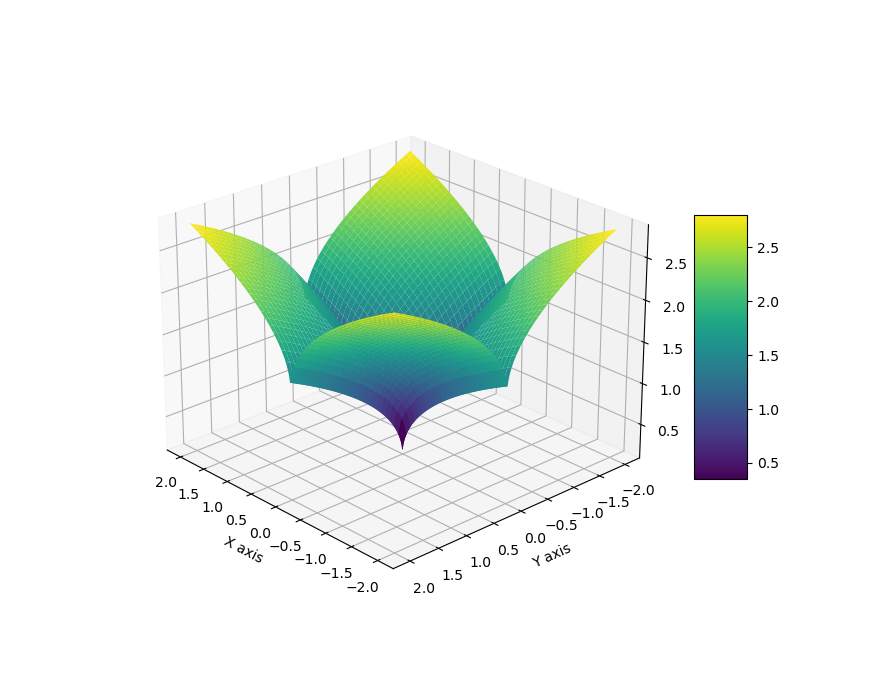
\includegraphics[width=0.5\linewidth]{./L0.5.png}\\
            \textbf{Upside:} L0.5 norm as shown in the graph is even pointier than L1 norm, which means that it can give
            even sparser results and select features more aggressively (filtering out even more small/zero features).\\
            \textbf{Downside:} Also from the graph we can see that the L0.5 norm is not convex, which means that it is hard
            to optimize and find the global minimum.
         \end{answer}
     \end{part}

     \begin{part}
        \begin{answer}
            \textbf{True,} when the step-size is too large, gradient decent can overshoot near the minimum and jump back and forth around the minimum and never converge.
         \end{answer}
     \end{part}
\newpage
     \begin{part}
        \begin{answer}
            \textbf{Advantage SGD has over GD:} SGD can converge significantly faster for large datasets since it updates the weights w.r.t. the gradient of a single randomly chosen sample, while GD requires calculating the gradient for the entire dataset.\\
            \textbf{Disadvantage of SGD has relative to GD:} SGD is more susceptible to noise/variance in the chosen sample and the decent path might be more volatile and might converge to a local minimum instead of the global minimum.
        \end{answer}
     \end{part}

     \begin{part}
        \begin{answer}
            Gradient descent is necessary for logistic regression because the loss function is convex but non-linear because of the sigmoid function and does not have a closed-form solution.
            While linear regression has convex function with a closed-form solution which makes gradient descent optional.
        \end{answer}
     \end{part}
\end{question}

%%%%%%%%%%%%%%%%%%%%%%%% Task 2 %%%%%%%%%%%%%%%%%%%%%%%%
\begin{question}{A2.}
    \begin{part}
       \begin{answer}
            \textbf{Non-negativity:} $\forall x \in \mathbb{R}^n$, $f(x) \ge 0$ holds because absolute values are non-negative ($|x_i| \ge 0$), and the sum of non-negative values 
             is also non-negative ($\sum_{i = 1}^{n} |x_i| \ge 0$), and this
            sum is 0 if and only if all the elements of $x$ are 0 (i.e. $x = 0$), thus $f(x) = 0$ iff $x = 0$ is also true. \\
            \textbf{Absolute scalability:} $\forall x \in \mathbb{R}^n, \forall a \in \mathbb{R}$, $f(ax) = |a|f(x)$ holds because by the definition of absolute value $|ax_i| = |a| |x_i|$ and therefore 
            $f(ax) = \sum_{i=1}^{n}|ax_i| = \sum_{i = 1}^{n}|a||x_i| = |a| \sum_{i = 1}^{n} |x_i|$ which is $|a|f(x)$.\\
            \textbf{Triangle inequality:} $\forall x,y\in\mathbb{R}^n, \;\; f(x + y) \le f(x) + f(y)$ holds because: \\
            for any $a,b \in \mathbb{R}$:\\
            \textit{Case 1 when $a,b$ has the same sign:}\\
            if $a,b \ge 0$ then $|a + b| = a + b = |a| + |b|$\\
            if $a,b < 0$ then $|a + b| = -(a + b) = -a - b = |a| + |b|$\\
            \textit{Case 2 when $a,b$ has different signs:}\\
            w.l.o.g. assume $a \ge 0, b \le 0$ then:\\
            if $|a| \ge |b|$ then $a + b \ge 0$ and thus $|a + b| = a + b \le a = |a| \le |a| + |b|$\\
            if $|a| < |b|$ then $a + b < 0$ and thus $|a + b| = -(a + b) = -a - b = |b| - |a| \le |b| \le |a| + |b|$\\
            Thus $|a + b| \le |a| + |b|$ holds for all $a,b \in \mathbb{R}$\\
            Following this, we can see that $f(x + y) = \sum_{i = 1}^{n} |x_i + y_i| \le \sum_{i = 1}^{n} |x_i| + |y_i| = f(x) + f(y)$\\\\
            Therefore $f(x) = \sum_{i = 1}^{n} |x_i|$ is a norm.
            
        \end{answer}
    \end{part}

    \begin{part}
        \begin{answer}
            Assume we have $x,y \in \mathbb{R}^2$ where $x = [1, 0]$ and $y = [0, 1]$, then \\
            $g(x + y) = (\sum_{i=1}^{2} |x_i+ y_i|^\frac{1}{2})^2 = (|x_1 + y_1|^\frac{1}{2} + |x_2 + y_2|^\frac{1}{2})^2
            = (|1+ 0|^\frac{1}{2} + |0 + 1|^\frac{1}{2})^2 = (1 + 1)^2 = 4 > 2 = 1^2 + 1^2 = (|x_1|^\frac{1}{2} + |x_2|^\frac{1}{2})^2 + (|y_1|^\frac{1}{2} + |y_2|^\frac{1}{2})^2 = (\sum_{i=1}^{2} |x_i|^\frac{1}{2})^2 + (\sum_{i=1}^{2} |y_i|^\frac{1}{2})^2 = g(x) + g(y)$\\
            Therefore $g(x) = (\sum_{i=1}^{n} |x_i|^\frac{1}{2})^2$ is not a norm.
         \end{answer}
     \end{part}
\end{question}

%%%%%%%%%%%%%%%%%%%%%%%% Task 3 %%%%%%%%%%%%%%%%%%%%%%%%
\begin{question}{A3.}
    \begin{part}[I]
       \begin{answer}
        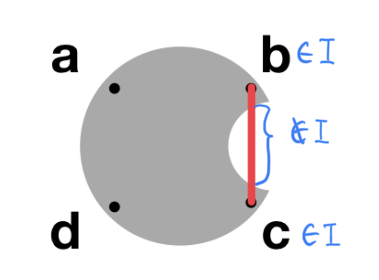
\includegraphics[width=0.45\linewidth]{i.png}\\
            \textbf{The set is not convex,} because as show in the graph, $b,c \in I$ but the line segment between $b$ and $c$ (i.e. $\lambda b + (1 - \lambda)c$) is not entirely in $I$ (the segment marked blue is not in grey-shaded region).
        \end{answer}
    \end{part}

    \begin{part}[II]
        \begin{answer}
            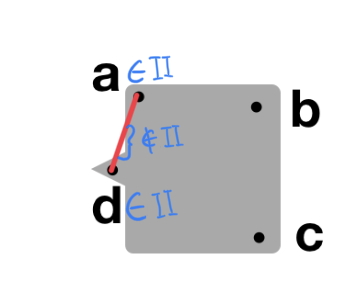
\includegraphics[width=0.45\linewidth]{ii.png}\\
            \textbf{The set is not convex,} because as show in the graph, $a,d \in II$ but the line segment between $a$ and $d$ (i.e. $\lambda a + (1 - \lambda)d$) is not entirely in $II$ (the segment marked blue is not in grey-shaded region).
         \end{answer}
     \end{part}
\end{question}

%%%%%%%%%%%%%%%%%%%%%%%% Task 4 %%%%%%%%%%%%%%%%%%%%%%%%
\begin{question}{A4.}
    \begin{part}
       \begin{answer}
            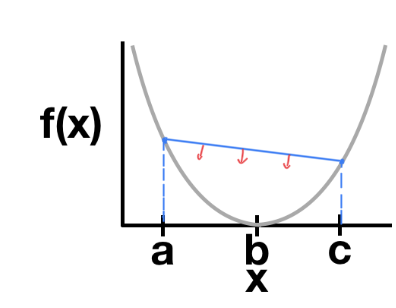
\includegraphics[width=0.45\linewidth]{./A.png}\\
            \textbf{The function is convex on the interval [a,c],} because as shown in the graph, the line segment between $(a,f(a))$ and $(c, f(c))$ (i.e. $\lambda f(a) + (1-\lambda)f(c)$)
            is above the function $f(x)$ for all $x \in [a,c]$ (i.e. $f(\lambda a + (1-\lambda)c) \le \lambda f(a) + (1-\lambda)f(c)$).
        \end{answer}
    \end{part}

    \begin{part}
        \begin{answer}
            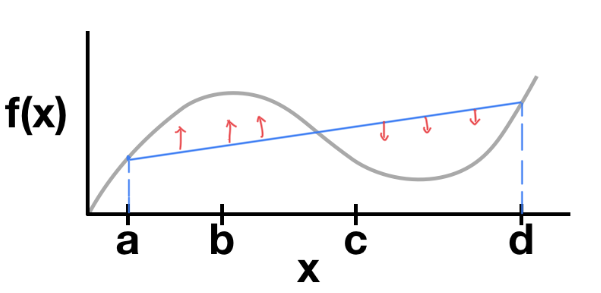
\includegraphics[width=0.45\linewidth]{./B.png}\\
            \textbf{The function is not convex on the interval [a,d],} because as shown in the graph the line segment between $(a,f(a))$ and $(b, f(b))$ (i.e. $\lambda f(a) + (1-\lambda)f(b)$)
            is below the function $f(x)$ for all $x \in [a,b]$ (i.e. $f(\lambda a + (1-\lambda)b) \ge \lambda f(a) + (1-\lambda)f(b)$), and $b \in [a,d]$.
         \end{answer}
     \end{part}
\end{question}
%%%%%%%%%%%%%%%%%%%%%%%% Task 5 %%%%%%%%%%%%%%%%%%%%%%%%
\begin{question}{A5.}
    \begin{part}
       \begin{answer}
            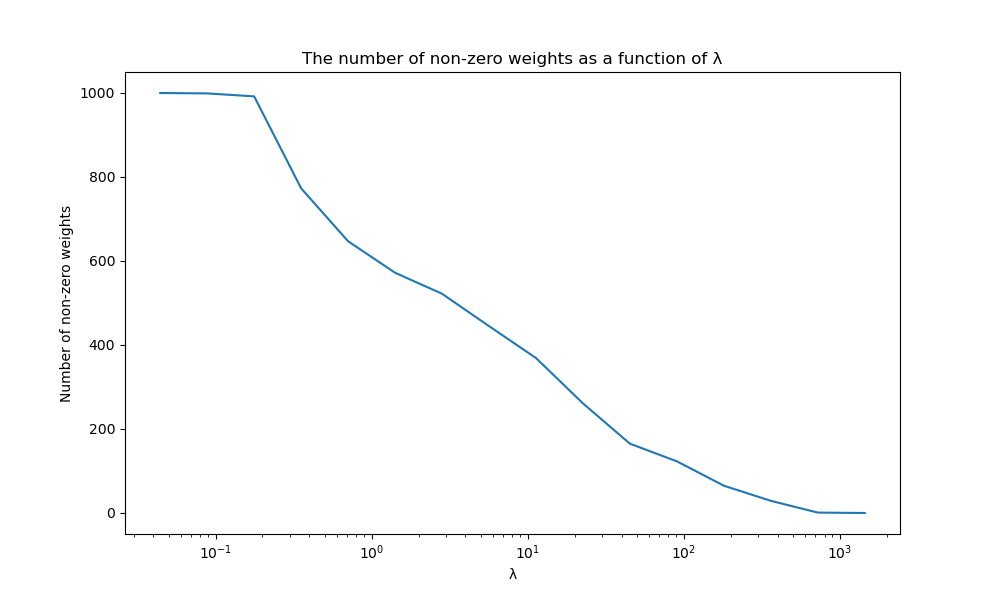
\includegraphics[width=0.85\linewidth]{A5a.png}
        \end{answer}
    \end{part}

    \begin{part}
        \begin{answer}
            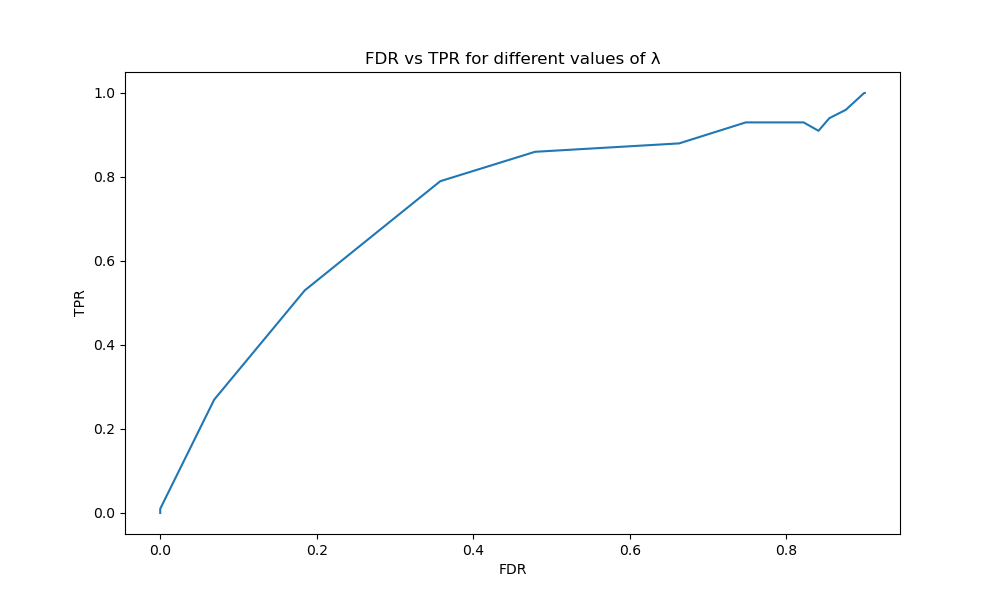
\includegraphics[width=0.85\linewidth]{A5b.png}
         \end{answer}
     \end{part}
\newpage
     \begin{part}
        \begin{answer}
            In the part a plot, as \( \lambda \) decreases, the number of non-zero weights in the model increases (higher $\lambda$ gives sparser results, lower $\lambda$ decreases sparsity).\\
            In the FDR vs TPR plot, as \( \lambda \) decreases (moving left to right in x-axis), the TPR increases (model identifies more features as relevant), and the FDR also increases (model includes more irrelevant features).
         \end{answer}
     \end{part}
\end{question}
%%%%%%%%%%%%%%%%%%%%%%%% Task 6 %%%%%%%%%%%%%%%%%%%%%%%%
\begin{question}{A6.}
    \begin{part}
       \begin{answer}
            \textbf{PctPopUnderPov:} percentage of people under the poverty level could be influenced by minimum wage laws, tax policies, welfare programs, job creation plans made by the government.\\
            \textbf{OfficAssgnDrugUnits:} number of officers assigned to special drug units could be influenced by the policy campaign of federal or state government (e.g. the war on drugs policy campaign).\\
            \textbf{PctPolicMinor:} percent of police that are minority could be influenced by the government's diversity hiring policy in law enforcement agencies.\\
            \textbf{PctUsePubTrans:} percent of people using public transit for commuting is highly influenced by government's decision on investments in public transit infrastructure.
        \end{answer}
    \end{part}

    \begin{part}
        \begin{answer}
            \textbf{LemasSwornFT:} a higher number of sworn full-time police officers could be a response to higher crime rates rather than a cause. As local decision makers may increase police presence in response to rising violence.\\
            \textbf{HousVacant:} a higher number of vacant households could be a result of rising local crime rates, as people may move out of the area to avoid crime.\\
            \textbf{LemasTotalReq:} total requests for police could rise in response to rising levels of violent crime.\\
            \textbf{RentLowQ:} high number of lower quartile rent housing could be a result of higher crime rates which may lower the demand for housing in the area and thus lower the rent prices.
         \end{answer}
     \end{part}

     \begin{part}
        \begin{answer}
            \includegraphics[width=0.85\linewidth]{A6c.png}
         \end{answer}
     \end{part}

     \begin{part}
        \begin{answer}
            \includegraphics[width=0.85\linewidth]{A6d.png}
        \end{answer}
     \end{part}

     \begin{part}
        \begin{answer}
            \includegraphics[width=0.85\linewidth]{A6e.png}
        \end{answer}
     \end{part}
\newpage
     \begin{part}
        \begin{answer}
            \textbf{Most positive:} PctIlleg (\% of kids born to never married), Value: 0.06164620954468405\\PctIlleg has the largest positive Lasso coefficient, which suggests that in our model, a higher percentage of children born to never married is correlated with the increase in violent crimes per capita.\\\\
            \textbf{Most negative:} PctKids2Par (\% of kids in family housing with two parents), Value: -0.04046680045005498\\
            PPctKids2Par has the most negative Lasso coefficient, which suggests that in our model, communities with a higher percentage of children living with both parents are correlated with lower rates of violent crimes per capita.
        \end{answer}
     \end{part}

     \begin{part}
        \begin{answer}
            Correlation $\ne$ causation. A large negative coefficient is only suggesting that higher values of agePct65up tend to show up with lower crime rates, and doesn't mean that increasing that feature will cause crime to decrease.
            People over 65 might have better financial autonomy to choose to live in safer neighborhoods, which could be a reason for the negative correlation.
        \end{answer}
     \end{part}
\end{question}
%%%%%%%%%%%%%%%%%%%%%%%% Task 7 %%%%%%%%%%%%%%%%%%%%%%%%
\begin{question}{A7.}
    \begin{part}
       \begin{answer}
            \begin{align*}
                \nabla_w J(w,b) &= \pderiv[]{}{x} (\frac{1}{n} \sum_{i=1}^n \log( 1 + \exp(-y_i (b + x_i^T w))) + \lambda ||w||_2^2)\\
                &= \frac{1}{n} \sum_{i=1}^n (\pderiv[]{}{x} (\log( 1 + \exp(-y_i (b + x_i^T w)))) + \pderiv[]{}{x}(\lambda w^\top w))\\
                &= \frac{1}{n} \sum_{i=1}^n \frac{-y_i x_i \exp(-y_i (b + x_i^T w))}{1 + \exp(-y_i (b + x_i^T w))} + 2\lambda w \tag{chain rule}\\
                &= \frac{1}{n} \sum_{i=1}^n -y_i x_i (1 - \frac{1}{1 + \exp(-y_i (b + x_i^T w))}) + 2\lambda w\\
                &= \frac{1}{n} \sum_{i=1}^n -y_i x_i (1 - \mu_i(w,b)) + 2\lambda w \tag{since $\mu_i(w,b) = \frac{1}{1 + \exp(-y_i (b + x_i^T w))}$}\\
                &= \boxed{-\frac{1}{n} \sum_{i=1}^n y_i x_i (1 - \mu_i(w,b)) + 2\lambda w}
            \end{align*}
            \begin{align*}
                \nabla_b J(w,b) &= \pderiv[]{}{b} (\frac{1}{n} \sum_{i=1}^n \log( 1 + \exp(-y_i (b + x_i^T w))) + \lambda ||w||_2^2)\\
                &= \frac{1}{n} \sum_{i=1}^n (\pderiv[]{}{b} (\log( 1 + \exp(-y_i (b + x_i^T w)))) + \pderiv[]{}{b}(\lambda w^\top w))\\
                &= \frac{1}{n} \sum_{i=1}^n \frac{-y_i \exp(-y_i (b + x_i^T w))}{1 + \exp(-y_i (b + x_i^T w))} + 0 \tag{chain rule}\\
                &= \frac{1}{n}  \sum_{i=1}^n -y_i (1 - \frac{1}{1 + \exp(-y_i (b + x_i^T w))})\\
                &= \frac{1}{n}  \sum_{i=1}^n -y_i (1 - \mu_i(w,b)) \tag{since $\mu_i(w,b) = \frac{1}{1 + \exp(-y_i (b + x_i^T w))}$}\\
                &= \boxed{-\frac{1}{n}  \sum_{i=1}^n y_i (1 - \mu_i(w,b))}
            \end{align*}
        \end{answer}
    \end{part}
\newpage
    \begin{part}
        \begin{answer}
            (i)Learning rate = 1e-1, epochs = 100, $\lambda = 1e-1$\\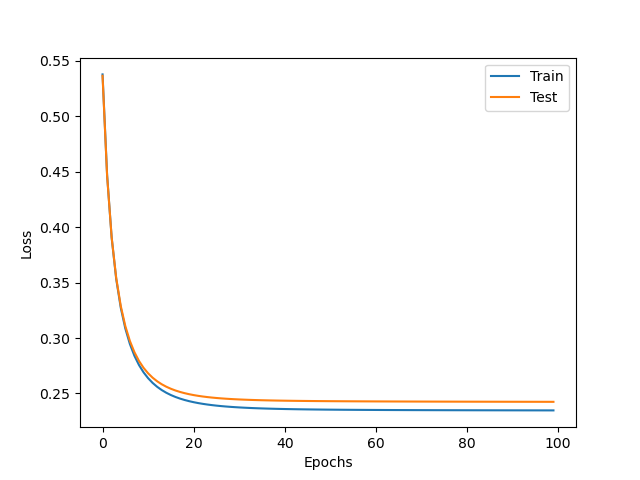
\includegraphics[width=0.85\linewidth]{a7bi.png}\\
            (ii)Learning rate = 1e-1, epochs = 100, $\lambda = 1e-1$\\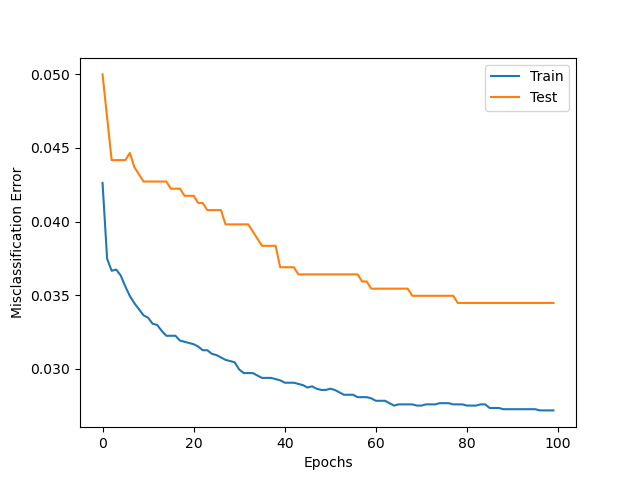
\includegraphics[width=0.85\linewidth]{a7bii.png}
         \end{answer}
     \end{part}

     \begin{part}
        \begin{answer}
            (i)Learning rate = 1e-5 (1e-4 times the learning rate of GD), epochs = 100, $\lambda = 1e-1$\\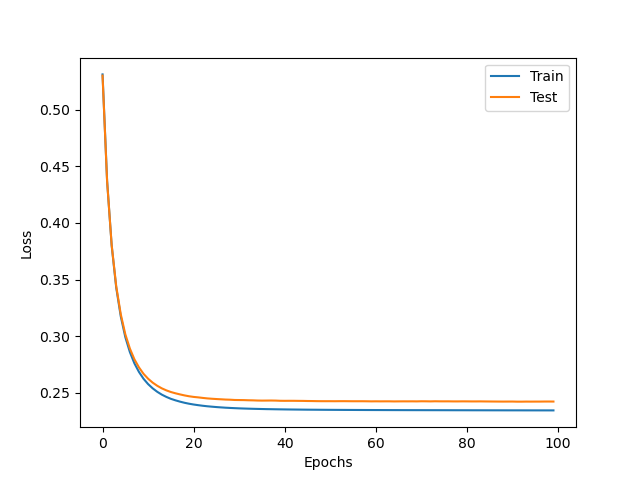
\includegraphics[width=0.85\linewidth]{a7ci.png}\\
            (ii)Learning rate = 1e-5 (1e-4 times the learning rate of GD), epochs = 100, $\lambda = 1e-1$\\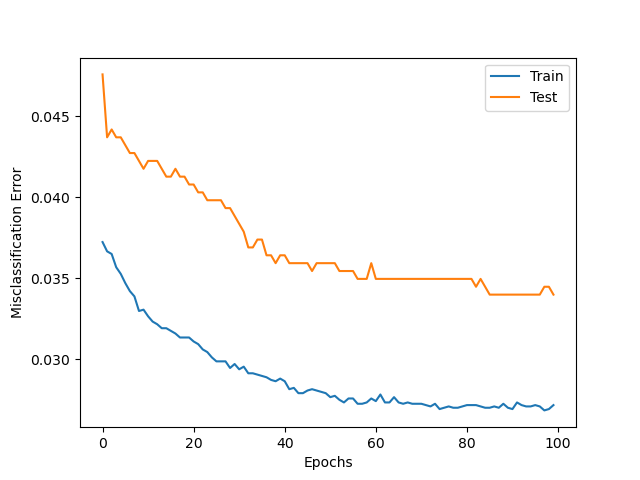
\includegraphics[width=0.85\linewidth]{a7cii.png}
         \end{answer}
     \end{part}

     \begin{part}
        \begin{answer}
            (i)Learning rate = 1e-3 (100 times the learning rate of batch size 1), epochs = 100, $\lambda = 1e-1$\\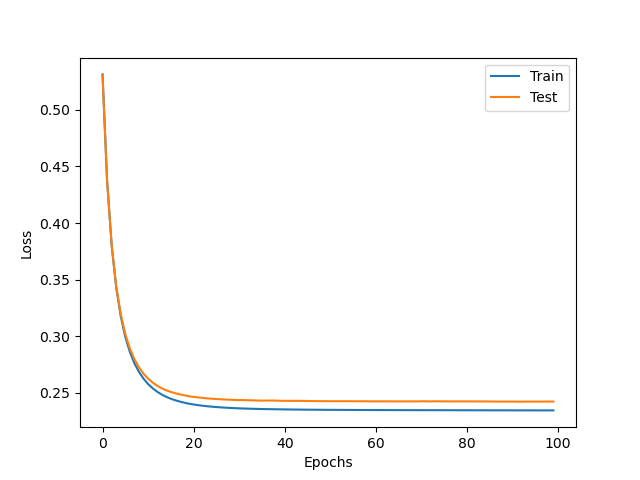
\includegraphics[width=0.85\linewidth]{a7di.png}\\
            (ii)Learning rate = 1e-3 (100 times the learning rate of batch size 1), epochs = 100, $\lambda = 1e-1$\\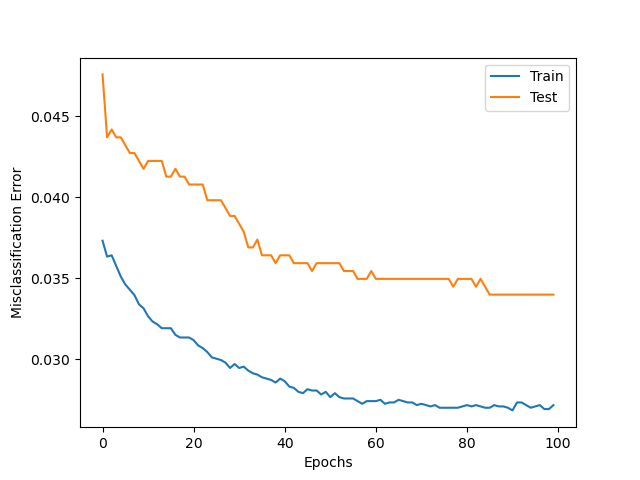
\includegraphics[width=0.85\linewidth]{a7dii.png}
        \end{answer}
     \end{part}

\end{question}
%%%%%%%%%%%%%%%%%%%%%%%% Task 8 %%%%%%%%%%%%%%%%%%%%%%%%
\begin{question}{A8.}
    \begin{part}
       \begin{answer}
            20 hours
        \end{answer}
    \end{part}
\end{question}
\end{document}
